\documentclass[xcolor={dvipsnames}]{beamer}
\usepackage{amsmath}
% \usepackage{beamerthemesplit} // Activate for custom appearance
\usepackage{hyperref}
\usepackage{ragged2e}
\usepackage{cancel}
%\usepackage{fancyvrb}
%\fvset{commandchars=\\\{\}}

\title{SQL}
\author{Schwartz}
\date{\today}


\begin{document}

\frame{\titlepage}






\frame
{
 \frametitle{Sizes of things}
 
 \vspace{.2em}
 
 \tiny
 \begin{tabular}{|l|lllll|}\hline
  & Binary   &   & Decimal  && Example\\\hline
Bit   & $2^0$ &   1 &                &        &      Binary (0 or 1) \\
Byte (B) & $2^3$ &  8 &          &             & \textcolor{red}{"S" = 01010011} \\ \hline
Kilobyte (KB) & $2^{10}$ & 1,024 &  $10^3$ & 1,000 & Word Document \\
Megabyte (MB) & $2^{20}$ & 1,048,567 & $10^6$ & 1,000,000 &  Digital Photo \\  
Gigabyte (GB) & $2^{30}$ & 1,073,741,824 & $10^9$ & 1,000,000,000 &  DVD  \\
Terabyte (TB) &  $2^{40}$ &   1,099,511,627,776 & $10^{12}$  & 1,000,000,000,000 &  Hard Drive  \\
Petabyte (PB) & $2^{50}$ &    1,125,899,906,842,624 & $10^{15}$  & 1,000,000,000,000,000 & Some of Facebook  \\ \hline
All Atoms  &            $2^{266}$ &  $\cdots$      &$10^{80}$      & $\cdots$ & Universe    \\
TSP routes &       $2^{329}$ & $(71-1)!/2$ &$10^{99}$ & $\cdots$& 71 cities  \\\hline
 \end{tabular}

\vspace{-1.4em}

\onslide<2->{
\huge
%\color{Maroon}
 \begin{tabular}{l}
 \tiny $\;\;$ \\
 Ascii is \\
 encoded \\
 as 8 bits $\;\;$ \\
 $\displaystyle \sum^7_{i=0} b_i 2^{i}$\\\\\\\\\\\\\\%$b_i \in \{0,1\}$\\\\\\\\\\\\\\
 \end{tabular}\color{black}\fbox{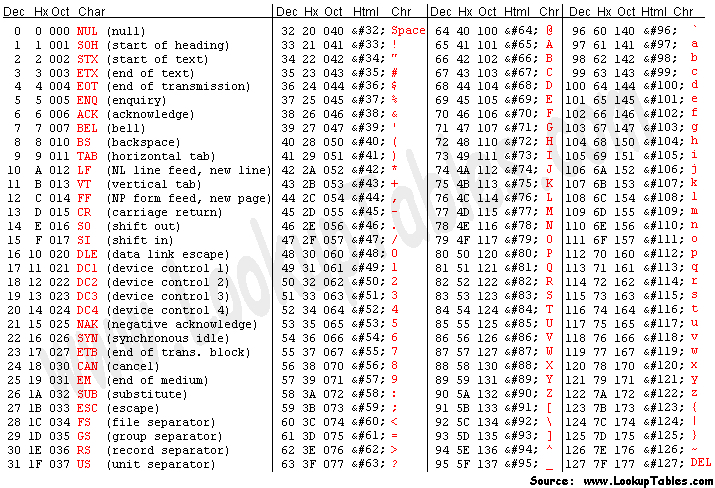
\includegraphics[width=3in]{stuff/asciifull.jpg} }}
 
}



\frame
{
\frametitle{Objectives}

\Large
\begin{enumerate}%[leftmargin=*]
\item Learn what a RDBMS is

\item \textcolor{gray}{Learn the ways tables can be joined}


\item Learn some \textcolor{gray}{postgre}SQL

\begin{itemize}
\item create, alter, insert-delete-update, and drop tables
\end{itemize}

\item Learn more \textcolor{gray}{postgre}SQL
\begin{itemize}
\color{gray}
\item SELECT
\item AS, DISTINCT
\item *, /, +, -, CONCAT, ROUND, CAST, COALESCE
\item WHERE, CASE WHEN THEN ELSE END
\item  $=$, $<$, $<=$, $>$, $>=$, $!=$, $<>$, AND, OR, BETWEEN, LIKE, IN 
\item NULL, IS NULL, IS NOT NULL
\item FROM/JOIN ON,  LEFT, RIGHT, FULL [OUTER]
\item GROUP BY, MAX, MIN, SUM, AVG, COUNT
\item HAVING, ORDER BY, LIMIT
\item (SELECT ...)
\end{itemize}

\item Practice, practice, practice...
\end{enumerate}
}


\frame
{
 \frametitle{Relational Database Management System (RDBMS)}

\Large 
\begin{itemize}
\item Efficient queries of data and relations therein 
\item<2-> \emph{Schema}: tables and typed data columns  
\begin{itemize}
\large 
\item \emph{Keys}: data relationships 
\end{itemize} 
%\item  \emph{Persistance}: non-volatile storage 
\item<3-> \emph{ACID}: reliability properties

\begin{itemize}
\large
\item[A:] Atomicity -- ``all or nothing''
\item[C:] Consistency -- ``remain in legal state''
\item[I:] Isolation -- ``appropriate independence''
\item[D:] Durability -- ``persistance'' (non-volatile storage)
\end{itemize} 
\item[]
\item<4-> psql $\quad\;\;\;$ \textbackslash l $\quad\;\;\;$ \textbackslash c $<$DB$>$ $\quad\;\;\;$ \textbackslash d [table] 
\end{itemize}
}



\begin{frame}[fragile]\frametitle{Schema}

\color{gray}
\begin{verbatim}
CREATE DATABASE dbname;
\end{verbatim}
\vspace{-2em}
\color{black}

\begin{verbatim}
CREATE TABLE users {
    id INTEGER PRIMARY KEY,
    name VARCHAR(255),
    age INTEGER,
    city VARCHAR(255),
    state VARCHAR(2)
}
\end{verbatim}

\begin{itemize}
\item<2-> Whitespace doesn't matter 
\item<2->[] (but it can help make code clearer)
\item<3-> Capitalization (often) doesn't matter 
\item<3->[] (but it can help make code clearer)
\item<4-> Don't look like a noob
\begin{itemize}
\item follow ubiquitous conventions
\item write beautiful looking code
\end{itemize}
\end{itemize}

\end{frame}


\begin{frame}[fragile]\frametitle{Schema \emph{efficiency} \textcolor{gray}{(referenced ``users" table on last slide!)}}

\begin{verbatim}
CREATE TABLE visits {
    id INTEGER PRIMARY KEY,
    created_at TIMESTAMP,
    user_id INTEGER REFERENCES users(id)
    -- place foreign keys on the "many" 
    -- side of a one-to-many relationship
};
\end{verbatim}


\vspace{3in}

\end{frame}	




\begin{frame}[fragile]\frametitle{Schema \emph{efficiency}}

\begin{verbatim}
CREATE TABLE visits {
    id INTEGER PRIMARY KEY,
    created_at TIMESTAMP,
    user_id INTEGER REFERENCES users(id)
    -- place foreign keys on the "many" 
    -- side of a one-to-many relationship
};
\end{verbatim}


\begin{columns}
\begin{column}{.005\textwidth}
${}$
\end{column}
\begin{column}{.5\textwidth}
\color{blue}
\begin{verbatim}
CREATE TABLE posts {
    id INTEGER PRIMARY KEY,
    title VARCHAR(255)
};
\end{verbatim}
\end{column}
\begin{column}{.5\textwidth}
\color{blue}
\begin{verbatim}
CREATE TABLE tags {
    id INTEGER PRIMARY KEY,
    tag VARCHAR(255)
};
\end{verbatim}
\end{column}
\end{columns}


\begin{verbatim}
CREATE TABLE posts_tags {
    post_id INTEGER REFERENCES posts(id),
    tag_id INTEGER REFERENCES tags(id)
    -- "Normalized" data only duplicates foreign keys 
};
\end{verbatim}

\end{frame}	




\begin{frame}
\frametitle{Schema \emph{efficiency} example}

\LARGE
Do you like \emph{this?}
\normalsize

\begin{figure}
\centering


\begin{tabular}{|l|l|}
\hline
My *new* Jawdins & \#fab\\
My *new* Jawdins & \#shoes\\
My *new* Jawdins & \#fashion\\
Subway shoes & \#shoes\\
Subway shoes & \#envy \\ \hline
\end{tabular}

\end{figure}

${}$\\${}$

\LARGE
Or do you like \emph{this?}
\normalsize

\begin{columns}
\begin{column}{.5\textwidth}


\begin{tabular}{|l|l|}
\hline
1& Tip-toein' in my Jawdins\\
2 & NYC Subway Shoes \\ \hline
\end{tabular}

\end{column}

\begin{column}{.15\textwidth}

\begin{tabular}{|l|l|}
\hline
1 & a \\
1 & b \\
1 & c \\
2 & b \\
2 & d \\ \hline
\end{tabular}

\end{column}
\begin{column}{.35\textwidth}

\begin{tabular}{|l|l|}
\hline
a & \#fab\\
b & \#shoes\\
c & \#fashion\\
d & \#envy \\ \hline
\end{tabular}

\end{column}
\end{columns}

\end{frame}	


\frame{
\frametitle{JOIN and \emph{normalization} quiz}

% 1. [INNER] JOIN
% 2. LEFT [OUTER] JOIN
% 3. RIGHT [OUTER] JOIN
% 4. FULL [OUTER] JOIN
% 5. "Home" inner joined with "Home"
% 6. Normalize this (3 things at least)

\vspace{-1em}

\hspace*{-1cm}\begin{columns}
\begin{column}{.25\textwidth}
\noindent   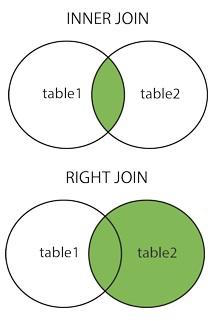
\includegraphics[width=1in]{stuff/joinA.jpg} \\
\noindent      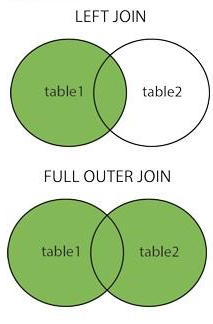
\includegraphics[width=1in]{stuff/joinB.jpg} 
\end{column}

\begin{column}{.3\textwidth}
   \scriptsize
  %    \\${}$\\
   \begin{tabular}{|l|l|l|}
   \hline 
 name & from & LL \\ \hline
ForesT & LA & T \\
JacK & VA & K \\
JamiE & CT & E \\
KatiE & CT & E \\
KeviN & NY &N \\
LaureN & NY &N \\
MichaeL & IL & L \\
RandalL & CA & L \\
RusselL & OH &L \\
TrevoR & NY &R\\ \hline
   \end{tabular}
   
 \normalsize
  
  \vspace{2.5em}
\onslide<2->{\textcolor{black}{Quiz: \emph{how many rows result from\\${}$\\}}} 

\onslide<3->{\textcolor{black}{Quiz: \emph{normalize \\the left table}}} 


    
\end{column}   
\begin{column}{.35\textwidth}
   \scriptsize
% \\  ${}$\\
   \begin{tabular}{|l|l|l|}
   \hline 
LL & place \\  \hline
N & CharlestoN  \\
E & NashvillE \\
E & Portland, ME \\
R & Portland, OR \\
H & PittsburgH \\ 
E & Sante FE \\ \hline
   \end{tabular}

\vspace{.4em}

\normalsize
\begin{itemize}
\item[]
\item[]
\item[]
\item[]
\item<2-> inner join?
\item<2-> right join?
\item<2-> left join?
\item<2-> outer join?
\end{itemize}   

      
   \end{column}   
   \end{columns}
  




   
}





\begin{frame}[fragile]\frametitle{Structured Query Language (SQL)}
SQL is used to interact with RDBMS, allowing one to 
\begin{itemize}
\item create tables \textcolor{gray}{(we saw this previously)}
\item alter tables
\item insert records
\item update records
\item delete records
\item query records within and across tables
\item[]
\end{itemize}

\color{white}\begin{verbatim}
CREATE [TEMPORARY] TABLE table AS (SELECT ...)
\end{verbatim}
\end{frame}


\begin{frame}[fragile]\frametitle{Structured Query Language (SQL)}

\vspace{.75em}

SQL is used to interact with RDBMS, allowing one to 
\begin{itemize}
\item \textbf{create tables} \textcolor{gray}{(we saw this previously)}
\item alter tables
\item insert records
\item update records
\item delete records
\item query records within and across tables
\item[]
\end{itemize}

\begin{verbatim}
CREATE DATABASE <dbname>;
CREATE [TEMPORARY] TABLE table AS <SQL query>;
\end{verbatim}
\end{frame}

\begin{frame}[fragile]\frametitle{Structured Query Language (SQL)}
SQL is used to interact with RDBMS, allowing one to 
\begin{itemize}
\item create tables \textcolor{gray}{(we saw this previously)}
\item \textbf{alter tables}
\item insert records
\item update records
\item delete records
\item query records within and across tables
\item[]
\end{itemize}

\begin{verbatim}
ALTER TABLE table [DROP/ADD/ALTER] column [datatype];
\end{verbatim}
\end{frame}

\begin{frame}[fragile]\frametitle{Structured Query Language (SQL)}
SQL is used to interact with RDBMS, allowing one to 
\begin{itemize}
\item create tables \textcolor{gray}{(we saw this previously)}
\item \textbf{alter tables}
\item insert records
\item update records
\item delete records
\item query records within and across tables
\item[]
\end{itemize}

\begin{verbatim}
DROP TABLE table;
\end{verbatim}
\end{frame}

\begin{frame}[fragile]\frametitle{Structured Query Language (SQL)}
SQL is used to interact with RDBMS, allowing one to 
\begin{itemize}
\item create tables \textcolor{gray}{(we saw this previously)}
\item alter tables
\item \textbf{insert records}
\item update records
\item delete records
\item query records within and across tables
\item[]
\end{itemize}

\begin{verbatim}
INSERT INTO table [(c1,c2,c3,...)] VALUES (v1,v2,v3,...);
\end{verbatim}
\end{frame}

\begin{frame}[fragile]\frametitle{Structured Query Language (SQL)}
SQL is used to interact with RDBMS, allowing one to 
\begin{itemize}
\item create tables \textcolor{gray}{(we saw this previously)}
\item alter tables
\item insert records
\item \textbf{update records}
\item delete records
\item query records within and across tables
\item[]
\end{itemize}

\begin{verbatim}
UPDATE table SET c1=v1,c2=v2,...WHERE cX=vX;
\end{verbatim}
\end{frame}

\begin{frame}[fragile]\frametitle{Structured Query Language (SQL)}
SQL is used to interact with RDBMS, allowing one to 
\begin{itemize}
\item create tables \textcolor{gray}{(we saw this previously)}
\item alter tables
\item insert records
\item update records
\item \textbf{delete records}
\item query records within and across tables
\item[]
\end{itemize}

\begin{verbatim}
DELETE FROM table WHERE cX=vX;
\end{verbatim}
\end{frame}

\begin{frame}[fragile]\frametitle{Structured Query Language (SQL)}
SQL is used to interact with RDBMS, allowing one to 
\begin{itemize}
\item create tables \textcolor{gray}{(we saw this previously)}
\item alter tables
\item insert records
\item update records
\item delete records
\item \textbf{query records within and across tables}
\item[]
\end{itemize}

\begin{verbatim}
SELECT.FROM.JOIN.ON.WHERE.GROUP BY.HAVING.ORDER BY.LIMIT 
\end{verbatim}
\end{frame}




\frame{
\frametitle{SQL \emph{order of operations}}

\begin{columns}
\begin{column}{.475\textwidth}

\begin{enumerate}
\LARGE 
\item<2-> FROM/JOIN/ON
\item<3-> WHERE
\item<4-> GROUP BY
\item<5-> ``aggregate''
\item<6-> HAVING
\item<7-> SELECT
\item<8-> ``transform''
\item<9-> ORDER BY
\item<10-> LIMIT
\end{enumerate}

\end{column}
\begin{column}{.55\textwidth}
\begin{enumerate}
\LARGE 
\item<2-> Merge Tables
\item<3-> Filter Rows
\item<4-> Partition Rows
\item<5-> Aggregate Rows
\item<6-> Filter Aggregations
\item<7-> Collect Columns
\item<8-> Transform Columns
\item<9-> Sort Rows
\item<10-> Print Subset
\end{enumerate}

\end{column}
\end{columns}


}




\frame{
\frametitle{Declarative Language: \emph{say what -- not how}}

The details of how things are actually done is just left up to SQL\\${}$\\${}$\\

My never ending query: \only<1>{\textcolor{red}{How do all queries start?}}\only<2-4>{\textcolor{red}{And then?}}\only<3-4>{\textcolor{red}{$\;$And then?}}\only<4>{\textcolor{red}{$\;$And then?}}\only<5-7>{\textcolor{red}{What about the "*", again?}}\only<8-14>{\textcolor{red}{What is the CASE syntax?}}\only<17-18>{\textcolor{red}{What's the difference between the aliases?}}\only<22-23>{\textcolor{red}{Now what?}}\only<24-28>{\textcolor{red}{How else?}}\only<35>{\textcolor{red}{What's this? What's next?}}\only<39>{\textcolor{red}{What's this? What's next?}}\only<41>{\textcolor{red}{This actually doesn't work. Why?}}\only<42>{\textcolor{red}{$\;\;\;\;\;\;\;\;$What's the difference?}}\only<43>{\textcolor{red}{Now What's the difference?}}\only<46>{\textcolor{red}{What's ``NULL''?}}\only<50-52>{\textcolor{red}{Do we need this?}}\only<51-52>{\textcolor{red}{$\;$ And this?}}\only<56-57>{\textcolor{red}{What's this?}}\only<58>{\textcolor{red}{Can we do this?}}\only<59>{\textcolor{red}{What are we doing here?}}\only<60>{\textcolor{red}{You will also see this sometimes}}\only<61>{\textcolor{red}{What's the difference here?}}\only<62-63>{\textcolor{red}{What's this? What's next?}}\only<65>{\textcolor{red}{Why this?}}\only<66>{\textcolor{red}{This?}}\only<67-68>{\textcolor{red}{What are we MISSING??}}\\${}$\\

\text{\only<2->{SELECT} \only<3-5>{*}\only<6-50>{c1,c2,}\only<51>{\textcolor{white}{c1,}c2,}\only<7->{CONCAT(\only<52>{MIN(}\only<53>{MAX(}\only<54->{AVG(}ROUND(100*c3/CAST(c2 AS REAL),2)\only<52->{)},'\%')}}\only<8->{,}

\text{$\quad$ \only<8->{CASE} \only<9->{WHEN} \only<10->{\textcolor{red}{$-$}}\only<11->{THEN} \only<12->{`a'} \only<13->{WHEN \textcolor{red}{$-$} THEN `b'} \only<14->{ELSE} \only<14->{`c'} \only<14->{END}
\only<15->{AS} \only<16->{clmn}}\\
\vspace{.5em}

$\quad$ \only<4->{FROM} \only<5->{table} \only<17>{AS }\only<17->{t}  
 \only<42->{LEFT }\only<42>{OUTER }\only<19->{JOIN} \only<20->{table2} \only<21>{AS }\only<21->{t2} 
\only<23->{ON} \only<24>{(table.id = table2.id2)}\only<25>{(t.id = t2.id2)}\only<26>{(id = id2)}\only<27>{id = id2}\only<28->{(t.id = t2.id2)}

\vspace{.5em}
\text{$\quad$ $\quad$ \only<29->{WHERE} \only<37->{(}\only<30->{t.c4}\only<31->{$\;<=\;$70} \only<32>{AND}\only<33->{OR} \only<34->{t2.c4} \only<35->{LIKE} \only<36->{`S\%'}\only<37->{)}\only<38-40>{ AND} \only<38-40>{clm }\only<39-40>{IN }\only<40>{(`a',`c')}}\only<41->{\cancel{\text{AND clm IN (`a',`c')}}}

$\quad\quad\quad\quad\quad\;\;\;\;$ \only<47->{(}\only<44->{AND \textcolor{red}{CASE - - - END}}  \only<45->{OR} \only<46->{t2.id2} \only<46->{IS NULL}\only<47->{)}

\vspace{.5em}
$\quad$ $\quad$ \only<49->{GROUP BY} \only<50->{c2}

\text{$\quad$ $\quad$ \only<55->{HAVING} \only<56-57>{AVE(1)}\only<58->{AVE(c1)} \only<56->{$>$} \only<59>{(SELECT  DISTINCT COUNT(*) FROM t3}\only<60>{(SELECT  DISTINCT COUNT(1) FROM t3}\only<61->{(SELECT  COUNT(DISTINCT c5) FROM t3}}

\text{\only<62->{\hspace{2.025in}WHERE c5 BETWEEN}\only<63->{\;`J' AND `M')}}

$\quad$ \only<64->{ORDER BY} \only<65>{c2}\only<66->{1}

$\quad$ \only<67->{LIMIT 1}\only<68->{\textcolor{red}{\textbf{;}}}
} 




\frame{
\frametitle{Conclusion (and SUPER HINT)}
\emph{It doesn't cost anything to}
\huge
\text{CREATE TABLE table AS (SELECT ...)}\\
\vspace{.5em}
\normalsize
\hspace{2.5em}\emph{use it, and then}
\Huge
\textcolor{white}{blahblah}\text{DROP TABLE table}


\Large
${}$\\${}$

\textcolor{Maroon}{And there's also that TEMPORARY thing that's\\\hspace{2.75in}totes cool/usable}

}


\end{document}

(SELF JOIN)
(SELECT)





{
\beamertemplatenavigationsymbolsempty

\frame
{
 \frametitle{Odd, even at best}

{
\fontfamily{<familyname>}\selectfont
\begin{quote}
\scriptsize
\justify
%In the 2015/16 season,   incredibly long
$\quad\quad$ Last year Leicester City was given  5000 to 1 odds to win the
English Premier League. Actually, these are the longest odds $\textrm{$\textbf{ever seen}$}$ for $\textrm{$\textbf{any}$}$ top tier sporting league...$\textrm{$\;\textbf{ever}$}$.  To put this in perspective, the current odds out of Vegas for ``the most unlikely team to win the 2016/2017 NFL season'' -- woefully disastrous Cleveland$^*$ Browns -- are 200 to 1. \\${}$\\

$\quad\quad$ Since the clubs inception in 1890, Leicester City has only managed to appear in the Premier league 10 seasons.  They had only been promoted the previous season and just barely escaped relegation in their final match that season. Only five teams -- Arsenal, Chelsea, Liverpool, Man. City, and Man. U. -- have held the trophy for the past 21 seasons.  \\${}$\\
%since 1995.
%In the ``modern era'' of Premier league 

$\quad\quad$Only a few stout souls put money down on Leicester City last year. %in 2015
And when Leicester City ($\textrm{\emph{literally against all odds}}$) won the premiership last season in absolutely stunning, unbelievable, and unprecedented fashion, those stout souls got paid. 
Everyone, that is, except for John Micklethwait.  John M has made the same bet -- 20 pounds (\$29) that Leicester will win their division -- every August for the past 20 years. Every year, that is, except this one. Last year he moved from London to New York and missed placing his bet. That's a pity for John M because if he \emph{had} made his bet he would have won 100,000 pounds, or \$145,355. \\${}$\\
%later that season 
%In 2015 

Overall, \$3,000 was bet on Leicester City last season. The $\textrm{\underline{unprecedented}}$ \$15,000,000 payout nearly bankrupted the bookmakers.  John M got \$0.\\${}$

\tiny 
$^*$Cleveland's 52-year championship drought  ended with the 2015/16 NBA season
%The Cavaliers 2015/16 NBA championship ended 
%last year \emph{just}
\end{quote}
}
}
}

\frame
{
 \frametitle{Odds}
$$\text{Odds} = \frac{p}{1-p} \Longrightarrow \text{p} = \frac{Odds}{1+Odds} \textcolor{gray}{\;= \frac{1}{1+Odds^{-1}}} $$

$$\textcolor{gray}{1-p = \frac{1}{1+Odds}}$$
}



\frame
{
\frametitle{Objectives}

\Large
\begin{enumerate}%[leftmargin=*]
\item Know why logistic regression is a thing
\item Know how to 
\begin{itemize}
\LARGE
\item execute a logistic regression, and
\item explain what it all means 
\end{itemize}
\item know ROC curves and such
\end{enumerate}

}


\frame{
\frametitle{Linear Regression}

\begin{columns}
\begin{column}{.5\textwidth}
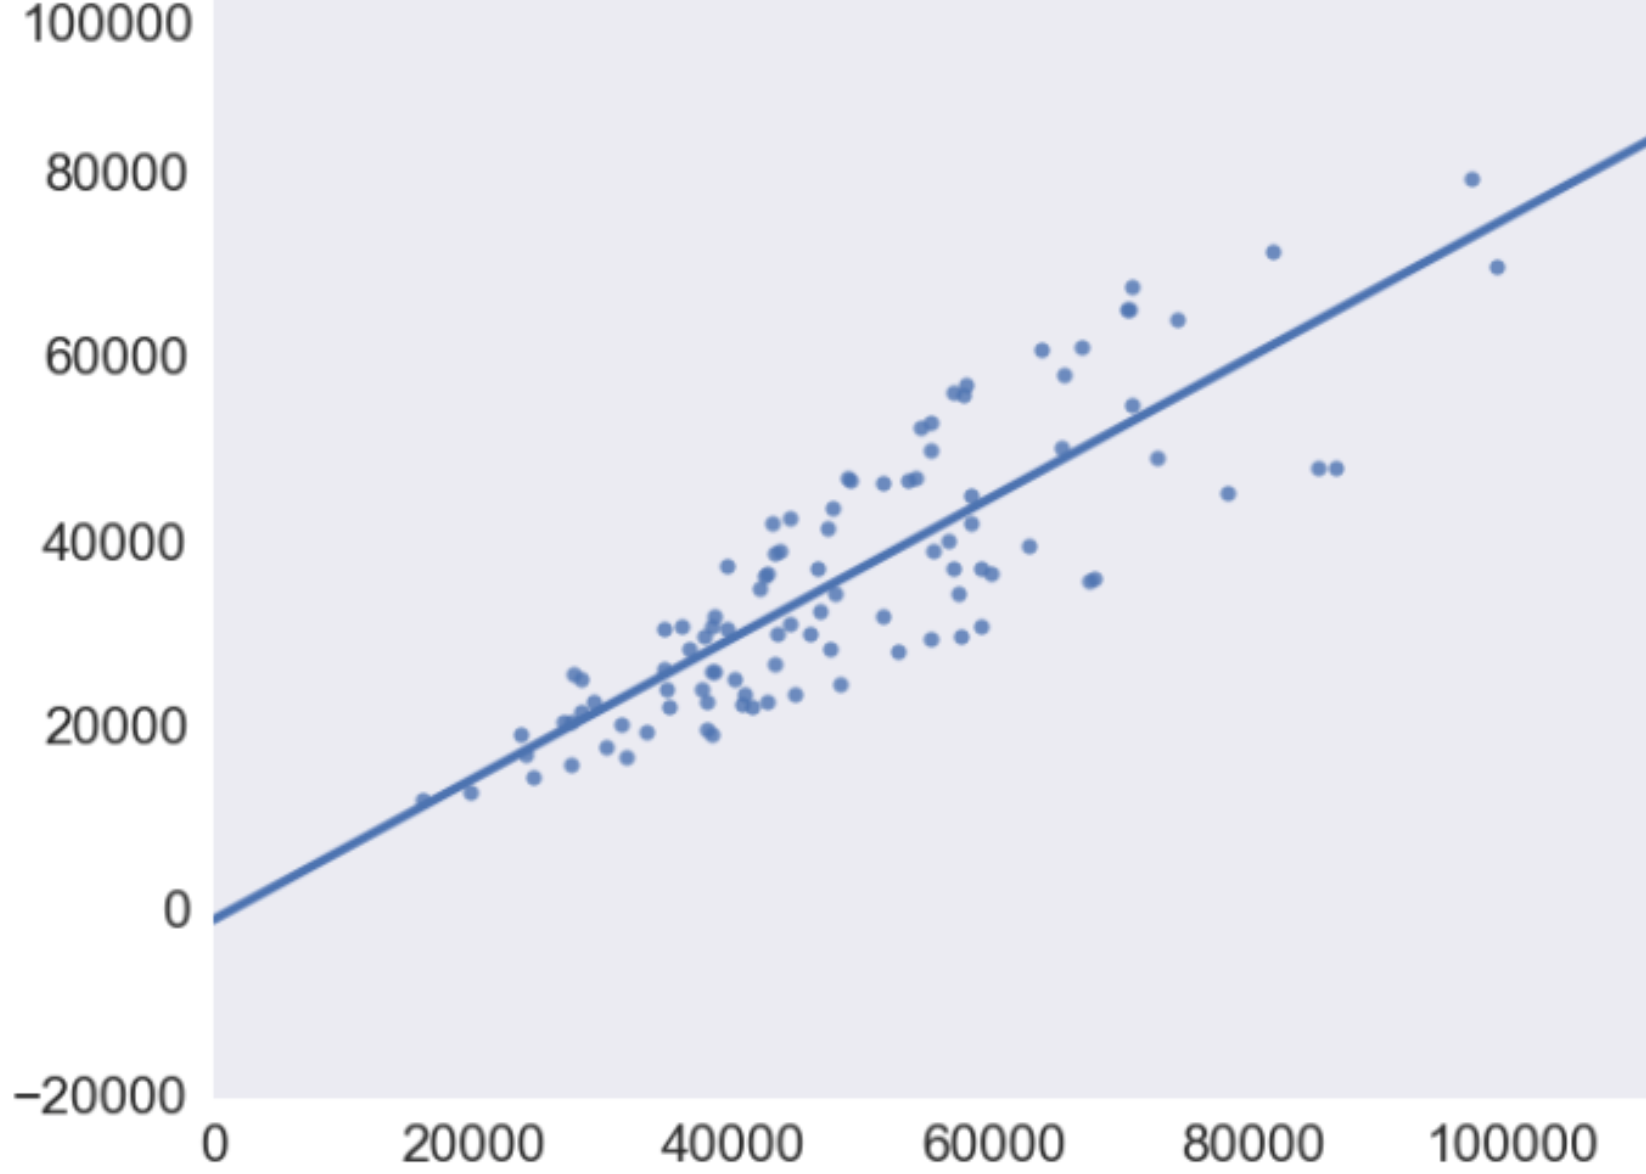
\includegraphics[width=2.1in]{log3.png}

\vspace{-.5em}
\huge 
\setlength{\leftmargini}{10pt}
\begin{itemize}
\item[]<2->
$$\text{Is this}$$
$$\text{satisfactory?}$$\\${}$
\end{itemize}

\end{column}
\begin{column}{.5\textwidth}

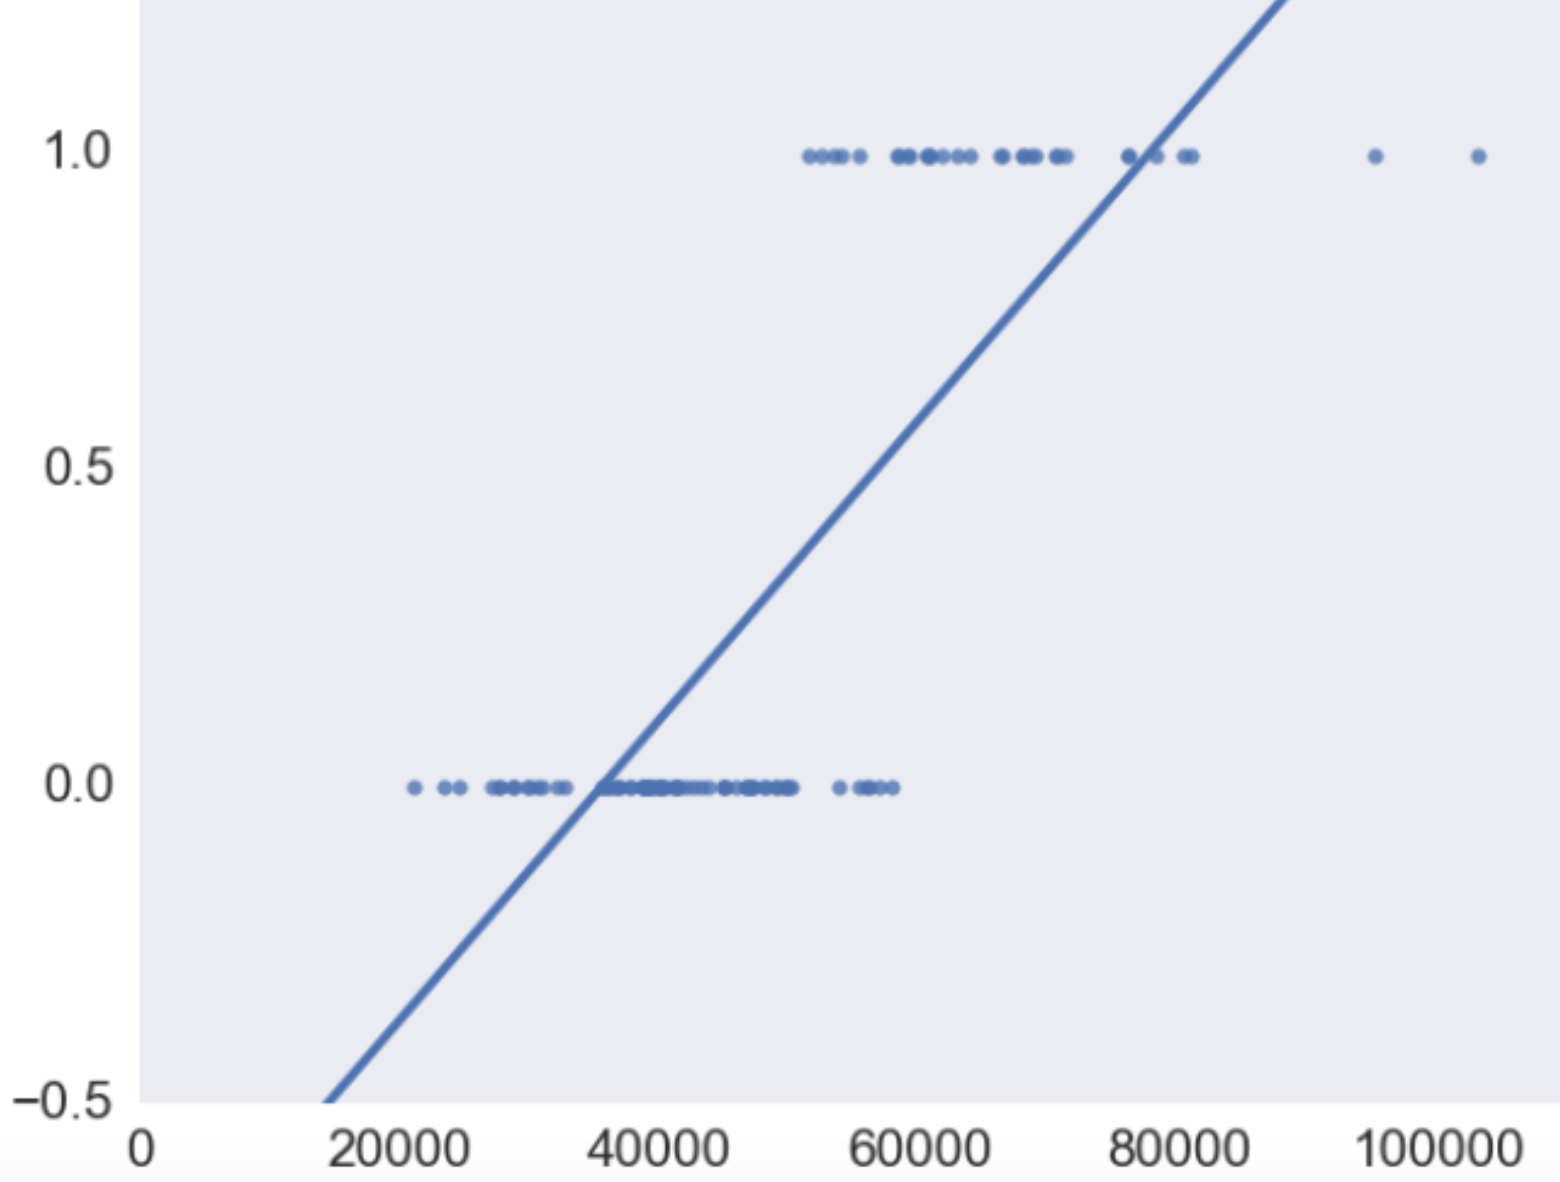
\includegraphics[width=2in]{log2.png}\\${}$

\vspace{-1em}
\setlength{\leftmargini}{0pt}
\begin{itemize}
\item[]<3->
\hspace{.4em}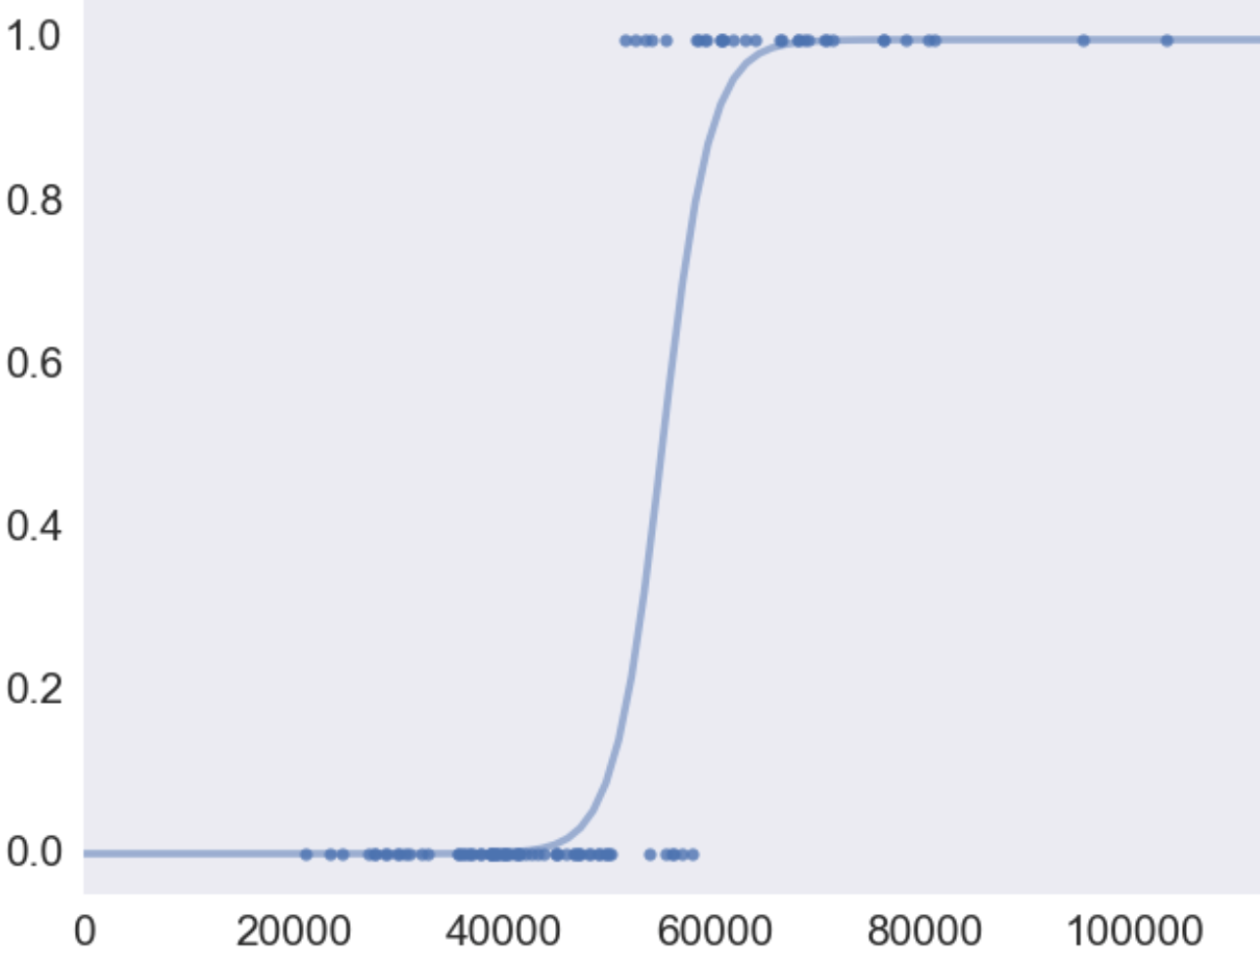
\includegraphics[width=1.925in]{log1.png}
\end{itemize}


\end{column}
\end{columns}
}




\frame
{
\frametitle{Link functions}

\begin{columns}
\begin{column}{.5\textwidth}
\begin{itemize}
\item The ``logit''  
$$g(p) = \log\left(\frac{p}{1-p}\right)$$
\item<2->  maps 
$$p \in {[}0,1{]} \mapsto Z \in \mathbb{R}$$\\${}$
\item<3->  Are we at odds about odds? 
\end{itemize}
\end{column}
\begin{column}{.5\textwidth}
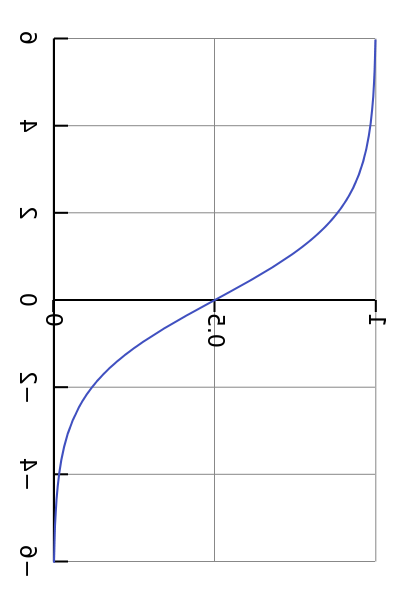
\includegraphics[width=2in]{Logistic-curve2.png}
\end{column}
\end{columns}
}



\frame
{
\frametitle{Logistic ``regression''}

\begin{itemize}
\item 
For a binary outcome $Y$, if we define  
$$\text{E}\left[Y\right] = \text{Pr}\left(Y=1\right) = g^{-1}(Z) = \frac{\exp(Z)}{1+\exp(Z)} = \frac{1}{1+\exp(-Z)}$$
$$\text{and let } Z =  \beta_0 + \beta_1x_{1} + \cdots + \beta_mx_m \textcolor{gray}{\; \in \mathbb R}$$  
\end{itemize}

\begin{figure}
\centering
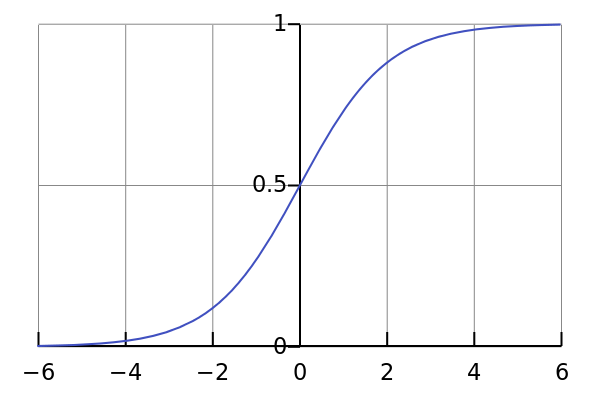
\includegraphics[width=3in]{Logistic-curve.png}

Standard logistic (sinusoid) function

\end{figure}
}

\frame
{
\frametitle{Logarithmic Scale}

\begin{itemize}
\item So
$$\text{Pr}(Y=1|x)  = \frac{1}{1 + e^{-(\beta_0 + \beta_1x_{1} + \cdots + \beta_nx_m )}}$$
\item<2-> And we can quickly see then that \\${}$

$\displaystyle \quad \frac{Pr(Y=1|x)}{Pr(Y=0|x)} \;\; = $
\vspace{-2.1em}
\item[]<3-> \hspace{9.2em}$\displaystyle \exp(\beta_0)\exp(\beta_1x_{1})\cdots\exp(\beta_mx_{m})$
\vspace{2.1em}
\item<4-> So for a 1-unit increase in $x_{j}$
\item[]<5->there is a  $\exp(\beta_j)$ multiplicative increase in \emph{the odds}
\item<6-> I.e., \emph{the odds} are linear in $x$ on a multiplicative, i.e.,
 odds increase with $x$ on a \emph{logorithmic} scale with base $\exp(\beta_j)$
\item<7-> The $log$ odds $log\left( \frac{Pr(Y=1|x)}{Pr(Y=0|x)} \right)$ are on a linear scale
\hspace*{2in}$\textcolor{gray}{(\beta_0 + \beta_1x_{1} + \cdots + \beta_nx_m)}$
\end{itemize}
}

\frame
{
\frametitle{The Odds Ratio (OR)}

\begin{itemize}
\item Equivalently, $\exp(\beta_j)$ is the \emph{odds ratio (OR)} 
between 1-unit differences in $x_{j}$ (e.g., 0 versus 1) when other $x$'s are constant
$$ \text{exp}(\beta_j) =  \frac{Pr(Y=1|x_j+1,x_{-j})/Pr(Y=0|x_j+1,x_{-j})}{Pr(Y=1|x)/Pr(Y=0|x)}  $$
\textcolor{gray}{
since 
\begin{align*}
{} & \frac{Pr(Y=1|x_j+1,x_{-j})}{Pr(Y=0|x_j+1,x_{-j})} \\
= {} & \exp(\beta_0)\exp(\beta_1x_{1})\cdots\exp(\beta_j(x_{j}+1))\cdots\exp(\beta_mx_{m})\\
= {} & \exp(\beta_0)\exp(\beta_1x_{1})\cdots\exp(\beta_jx_{j})exp(\beta_j)\cdots\exp(\beta_mx_{m})\\
\text{and} {} & \\
{} & \frac{Pr(Y=1|x)}{Pr(Y=0|x)}  \\
= {} & \exp(\beta_0)\exp(\beta_1x_{1})\cdots\exp(\beta_jx_{j})\cdots\exp(\beta_mx_{m}) 
\end{align*}}
\vspace{-.75em}
\item<2-> So $\beta_j$ is the change in $log(OR)$ for one unit changes in $x_j$...
\item[]
\end{itemize}
}


\frame
{
\frametitle{Logistic Regression \emph{Likelihood} and \emph{Deviance}}

\begin{itemize}
\item Likelihood 
$$\prod \left(\frac{1}{1+e^{-\textbf{x}_i^T\beta }}\right)^{Y_i} \left(\frac{1}{1+e^{\textbf{x}_i^T\beta}}\right)^{1-Y_i} $$\\${}$
\item<2-> Deviance 
\begin{align*}
D_M ={} & -2\left( \text{log}f(\textbf{Y}|\hat \theta^M) - \text{log}f(\textbf{Y}|\textbf{Y})\right) \\
\sim   {} &  \chi^2_{n-p-1} \\ 
{}\\
n  = {} &  \text{sample size}\\
k  = {} & \text{number of parameters in model }M\\
f(\textbf{Y}|\textbf{Y}) = {} &  \text{saturated model ($\textbf{Y}$ perfectly predicted)}
\end{align*}
\end{itemize}

}


\frame
{
\frametitle{More Deviance}

\begin{itemize}
\item In logistic regression \\
$D_M = -2\left( \text{log}f(\textbf{Y}|\hat \theta^M) - \text{log}f(\textbf{Y}|\textbf{Y})\right) =$\\${}$
\item<2->[]
\hspace{-3em}$-2 \sum  Y_i log (p_i) + (1-Y_i) log (1-p_i) -  \textcolor{pink}{Y_i log (Y_i) - (1-Y_i) log (1-Y_i)}$ 
\item[]
\item<3->[] \textcolor{gray}{\text{[show this]}}\\${}$

\item<4-> In linear regression 
\begin{align*}
D_M = {}& \frac{RSS}{\sigma^2}\quad\quad\quad\quad\;\; \textcolor{gray}{\text{[show this]}} \\ %(n-k) \frac{1}{n-k} 
= {}& \frac{\sum (Y_i - \hat Y)^2}{\sigma^2} \textcolor{gray}{\;=  (n-p-1) \frac{s^2}{\sigma^2}} \sim \chi^2_{n-p-1}
\end{align*}

\item[]<5-> 
\hspace{-1em}$\textcolor{gray}{[\text{what are \emph{residuals}?}]} \quad \onslide<6->{\textcolor{gray}{[\text{what are \emph{residuals} in logistic regression?}]}}$

\end{itemize}
}




\frame
{
\frametitle{Fitting Logistic Regression}

\begin{itemize}
\item MLE
$$\underset{\beta}{\text{max}} \prod \left(\frac{1}{1+e^{-\beta x}}\right)^{Y_i} \left(\frac{1}{1+e^{\beta x}}\right)^{1-Y_i}$$
$$\Longleftrightarrow$$
$$\underset{\beta}{\text{min}} \; D_\beta = \underset{\beta}{\text{max}} \left( \text{log}f(\textbf{Y}|\beta) - \text{log}f(\textbf{Y}|\textbf{Y})\right)$$

\item<2-> Closed form solution not available (like with linear regression)
\begin{itemize}
\item Optimization done via Newton-Rhapson or Gradient Decent
\end{itemize}

\item<3-> Convergence difficulties will be encountered if 
\begin{itemize}
\item too many features $(n/p < 10)$ or data is sparse/imbalanced 
\end{itemize}

\item<4-> Coefficient standard errors will be compromised when 
\begin{itemize}
\item predicted probabilities approach 1 or 0 (separated classes)
\item There is covariate multicollinearity (like linear regression)
\end{itemize}

\item<5-> What if, for some $\lambda$,  we choose $\beta$ to minimize
$$ -\prod \left(\frac{1}{1+e^{-\textbf{x}^T_i\beta}}\right)^{Y_i} \left(\frac{1}{1+e^{\textbf{x}^T_i\beta}}\right) + \lambda ||\beta||^2? $$

\end{itemize}
}


\frame
{
\frametitle{Fitting Logistic Regression}

\begin{itemize}
\item MLE
$$\underset{\beta}{\text{max}} \prod \left(\frac{1}{1+e^{-\beta x}}\right)^{Y_i} \left(\frac{1}{1+e^{\beta x}}\right)^{1-Y_i}$$
$$\Longleftrightarrow$$
$$\underset{\beta}{\text{min}} \; D_\beta = \underset{\beta}{\text{max}} \left( \text{log}f(\textbf{Y}|\beta) - \text{log}f(\textbf{Y}|\textbf{Y})\right)$$

\item Closed form solution not available (like with linear regression)
\begin{itemize}
\item Optimization done via Newton-Rhapson or Gradient Decent
\end{itemize}

\item Convergence difficulties will be encountered if 
\begin{itemize}
\item too many features $(n/p < 10)$ or data is sparse/imbalanced 
\end{itemize}

\item Coefficient standard errors will be compromised when 
\begin{itemize}
\item predicted probabilities approach 1 or 0 (separated classes)
\item There is covariate multicollinearity (like linear regression)
\end{itemize}

\item What if, for some $\lambda$,  we choose $\beta$ to minimize
$$ -\prod \left(\frac{1}{1+e^{-\textbf{x}^T_i\beta}}\right)^{Y_i} \left(\frac{1}{1+e^{\textbf{x}^T_i\beta}}\right) + \lambda |\beta|_1? \;\;$$

\end{itemize}


% minimize AIC/BIC (you see that/why?)
% when doing regression talk about types categorical, continuous, indicator

% odds ratio: "this many times more likely"

% uses -- see uses slides

% roc -- why is that worse than random guessing?
}




\frame
{
\frametitle{Pseudo $R^2$}

\begin{itemize}
\item McFadden's \emph{pseudo} $R^2 = 1 - D_M/D_0$
\item[]<2-> Proportion of deviance explained
\item[]
\item<3-> Compare to linear model $R^2 = 1 - RSS/TSS$
\item[]<4-> Proportion of variance explained
\item[]
\item<5->
\url{http://www.ats.ucla.edu/stat/mult_pkg/faq/general/Psuedo_RSquareds.htm}
\end{itemize}
}

\frame
{
\frametitle{Model Comparison}

\begin{itemize}
\item[] \textcolor{gray}{Remember, $D_M = -2(log f(\textbf{Y}|\hat \theta_M) - log f(\textbf{Y}|\textbf{Y}))$} 
\item<2-> Model comparison can be done using
$$D_R - D_F = -2\left( \text{log}f(Y|\hat \theta^R) - \text{log}f(Y|\hat \theta^F)\right) \overset{\tiny approx.}{\sim} \chi^2_k$$ 
where model $R$ is nested in model $F$ with $k$ fewer parameters
\item[] 
\item<3->
For \emph{non-nested} models, compare
\begin{align*}
AIC :{}& -2 \text{log}f(Y|\hat \theta) + 2k \\
BIC :{}& -2 \text{log}f(Y|\hat \theta) + k \text{log}(n) 
\end{align*}
\end{itemize}
}

\frame
{
\frametitle{Uses for logistic regression}

\begin{itemize}
\item<2-> Predict probabilities
\item<3-> Identify variables associated with outcomes
\item<4-> Classify outcomes (based on probabilities)
\item[]
\item<5-> \textcolor{gray}{Balancing comparison groups on \emph{propensity scores} Pr($T|x$) controls bias from group covariate composition differences} 

\end{itemize}
}



\frame
{
\frametitle{Confusion Matrix}

\begin{figure}
\centering
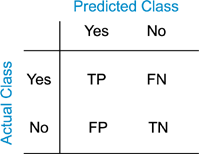
\includegraphics[width=2.5in]{confusionmatrix.png}
\end{figure}

\begin{itemize}
\item[]<2-> \hspace*{.8in}What is Type I and Type II error?
\end{itemize}

}


\frame
{
\frametitle{Sensitivity \& Specificity}

\begin{itemize}
\item Sensitivity:  \% of ``true $H_a$''  tests \underline{we correctly call} $\left(\frac{TP}{TP+FN}\right)$
\begin{itemize}
\item[] ``Are we \textbf{sensitive} to variations from $H_0$?''
\item[]
\item<2-> Also called \emph{True Positive Rate}
\end{itemize}
\item[]
\item<3-> Specificity:  \% of ``true $H_0$''  tests \underline{we correctly call} $\left(\frac{TN}{TN + FP}\right)$
\begin{itemize}
\item[]<3-> ``Are we \textbf{specific} about what $H_0$ means?''
\item[]
\item<4-> Also called \emph{True Negative Rate}
\item<4-> The related \emph{False Positive Rate} is $\left(\frac{FP}{TN+FP}\right)$
\end{itemize}
\item[]
\item<5-> the power of a test is Pr(Reject $H_0$ $|$ $H_a$ True) 
\item<5-> $\alpha$-significance level is Pr(Reject $H_0$ $|$ $H_0$ True)
\item<6-> \textbf{Are} power \textbf{and} $\alpha$ \textbf{Sensitivity and Specificity?}
\item<7-> \textbf{Are} Type I \textbf{and} Type II \textbf{Sensitivity and Specificity?}
\end{itemize}
}


\frame
{
\frametitle{ROC/AUC}


\begin{figure}
\centering
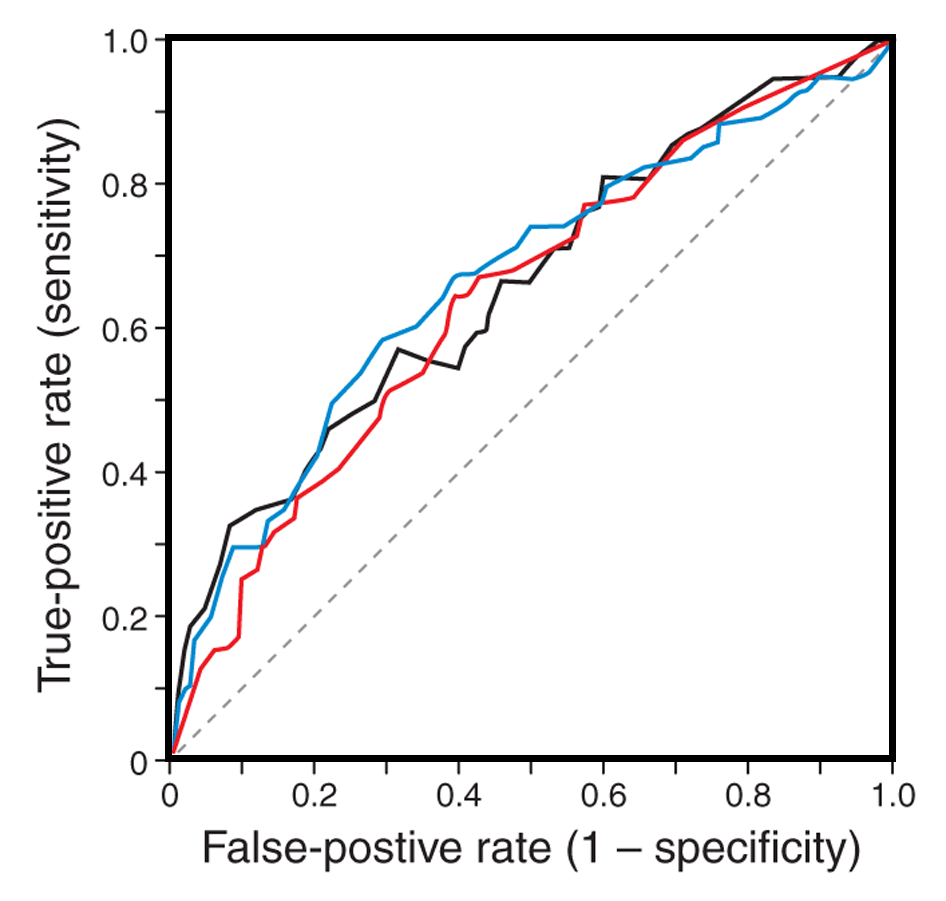
\includegraphics[width=2.5in]{roc.png}
\end{figure}
\vspace{-1em}
\url{https://www.youtube.com/watch?v=JAQC59ArFJw}
\url{https://www.youtube.com/watch?v=bhvvxNUbIpo}\\
\textcolor{gray}{**Notice how this is dependent upon the ``+'' and ``-'' \emph{populations}} 

}
% a video here would be rad... we'llp... I guess I'll just draw it...

\frame
{
\frametitle{Precision, False Discovery Rate, and Accuracy}

\begin{itemize}
\item Precision:  \% of \textbf{positives} \underline{we correctly call} $\left(\frac{TP}{TP+FP}\right)$
\begin{itemize}
\item ``How \textbf{precise} are we when we reject $H_0$?''
\item Also called \emph{Positive Predicted Value}
\end{itemize}
\item<2-> FDR:  \% of \textbf{positives} \underline{we \textbf{incorrectly} call} $\left(\frac{FP}{TP+FP}\right)$
\begin{itemize}
\item<2-> False Discovery Rate: ``What's our significant tests error rate?''
\item[]<3-> \emph{VERY} useful concept of multiple testing contexts
\item[]<3-> a.k.a. for a \emph{multiplicity adjustment} (where it's called a q-value)
\end{itemize}
\item<4-> Accuracy:  \% of tests we \underline{we correctly call} $\left(\frac{TP+TN}{Total}\right)$
\begin{itemize}
\item ``Do we call hypotheses accurately?''
\end{itemize}
\end{itemize}
\vspace{-10pt}
\onslide<5->{\begin{figure}
\centering
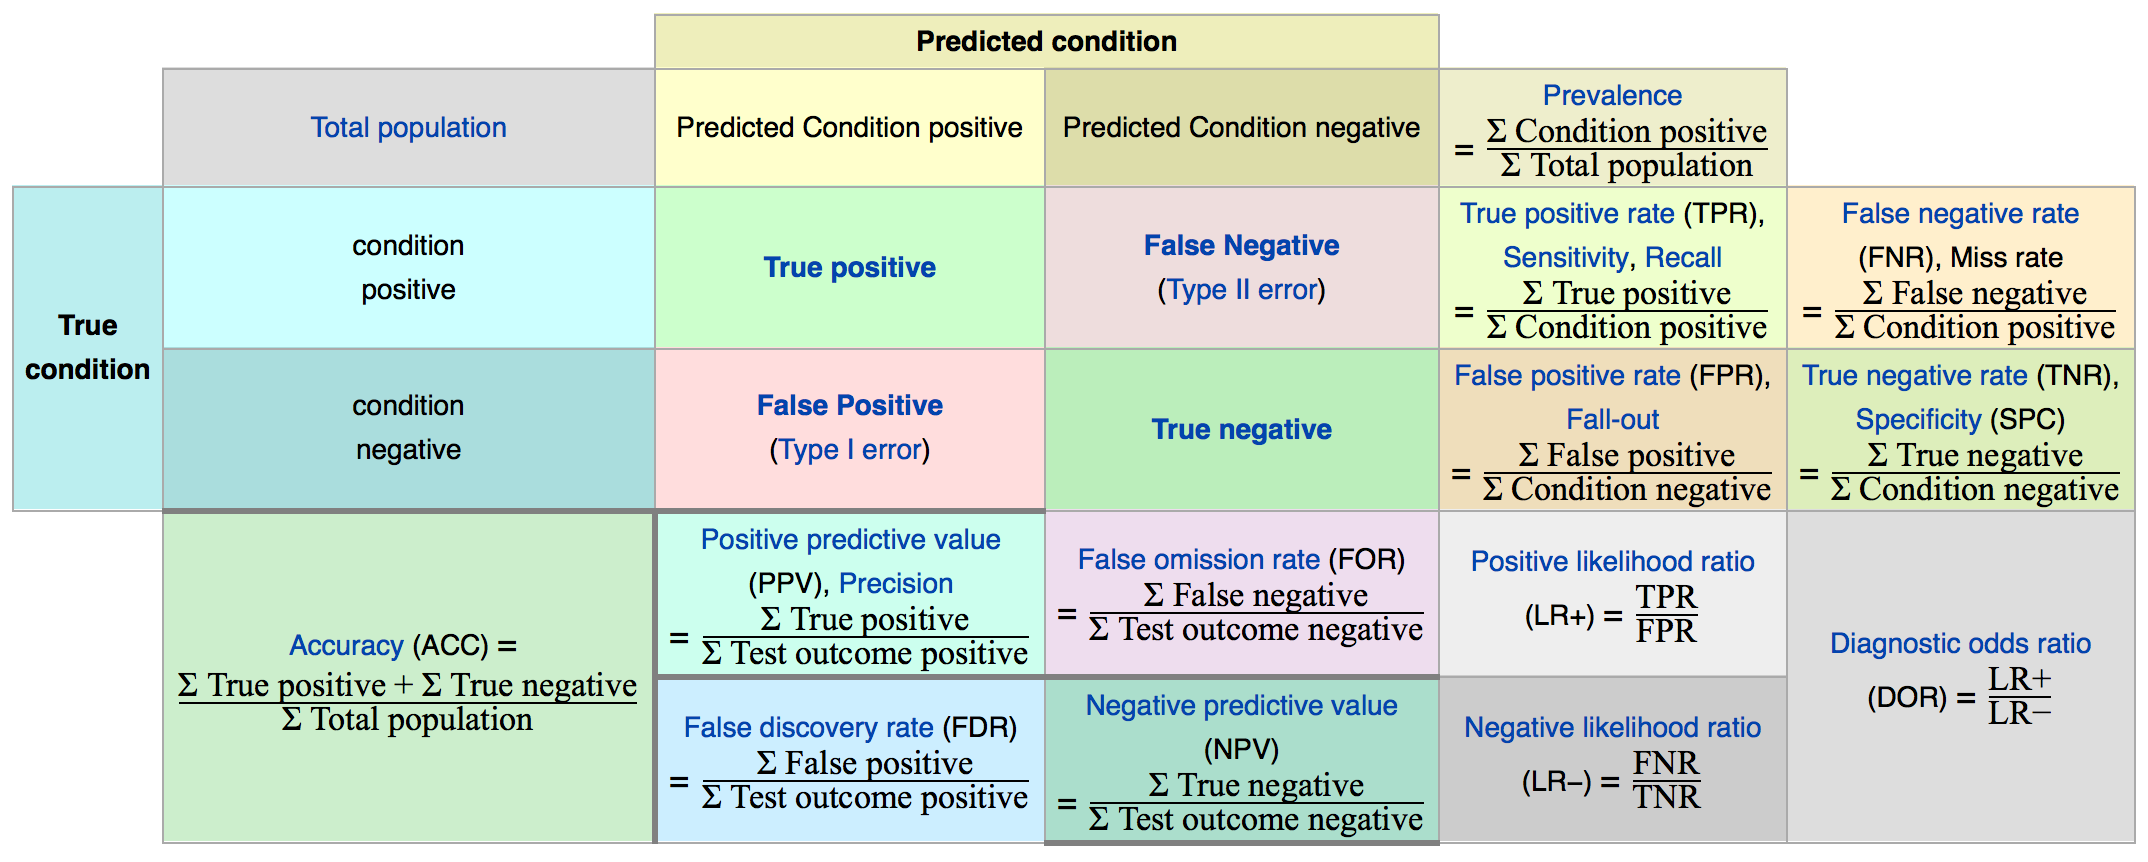
\includegraphics[width=4in]{terminology.png}

\tiny
Thanks, Wiki!
\end{figure}}

}


\end{document}



\begin{column}{.2\textwidth}
   \scriptsize
  %    \\${}$\\
   \begin{tabular}{|l|l|}
   \hline 
 Name & From \\ \hline
Katie & CT \\
Lauren &  \\
Michael & \\
Trevor &   \\ 
Will &   \\ \hline
   \end{tabular}
\end{column}   
\begin{column}{.35\textwidth}
   \scriptsize
% \\  ${}$\\
   \begin{tabular}{|l|l|l|}
   \hline 
Name &       Best Invention EVAR \\ \hline
Chris & Motocross \\
Jon & Lightbulbs \\
Katie &   \\
Katie & Rockets \\
Michael & Kiteboards \\
Scott &  \\
Trevor &  \\
Will & Education Systems \\ \hline
   \end{tabular}
   \end{column}   
   \end{columns}

